\input{../../style/preamble}
\input{../../latex-math/basic-math}
\input{../../latex-math/basic-ml}
\input{../../latex-math/ml-bagging.tex}
\input{../../latex-math/ml-boosting.tex}
\input{../../latex-math/ml-trees.tex}

\newcommand{\titlefigure}{figure_man/split-finding02.png}
\newcommand{\learninggoals}{
  \item Understand different ways gradient boosting can be made more efficient
  \item Learn how split finding can be sped up and parallelized
}

\title{Introduction to Machine Learning}
\date{}

\begin{document}

\lecturechapter{XGBoost}
\lecture{Introduction to Machine Learning}

% sources: https://homes.cs.washington.edu/~tqchen/pdf/BoostedTree.pdf
% sources: https://towardsdatascience.com/boosting-algorithm-xgboost-4d9ec0207d
% sources: https://devblogs.nvidia.com/parallelforall/gradient-boosting-decision-trees-xgboost-cuda/

\begin{vbframe}{Motivation}

\pkg{XGBoost} (short for eXtreme Gradient Boosting) is an open-source and scalable tree boosting system \textbf{(Chen and Guestrin 2016)}.

\lz

\begin{itemize}
  \item Efficient implementation in \emph{C++} with interfaces to many other programming languages.
  \item Parallel approximate split finding.
  \item Additional regularization techniques.
  \item Feature and Data subsampling.
  \item Cluster and GPU support.
\end{itemize}

\lz

\pkg{XGBoost} (and related implementations Catboost and LightGBM) are highly optimized and powerful machine learning frameworks and often achieve top performance in benchmarks and machine learning challenges.


\end{vbframe}

\begin{frame}{Regularization}

  \pkg{XGBoost} uses a risk function with 3 regularization terms:

  \begin{multline*}
    \riskr^{[m]} = \sum_{i=1}^{n} L\left(\yi, \fmd(\xi) + \bmm(\xi)\right)\\
     + \lambda_1 J_1(\bmm) + \lambda_2 J_2(\bmm) + \lambda_3 J_3(\bmm),
  \end{multline*}

  \lz

  with $J_1(\bmm) = T^{[m]}$ the number of leaves in the tree to penalize tree depth.

  \lz

  $J_2(\bmm) = \left\|\mathbf{c}^{[m]}\right\|^2_2$ and $J_3(\bmm) = \left\|\mathbf{c}^{[m]}\right\|_1$ are $L2$ and $L1$ penalties of the terminal region values $c_t^{[m]}, t=1,\dots,T^{[m]}$.

\end{frame}


\begin{vbframe}{Tree Growing}

  \pkg{XGBoost} grows trees with a maximum depth \texttt{max\_depth}.

  \lz

  Trees are fully expanded and leaves are split even if no improvement in risk can be achieved.

  \lz

  Only after the tree is fully expanded each split that did not improve the risk is pruned.

  \begin{figure}
    \includegraphics[trim=0 260 230 20, clip, width=\textwidth,page=2]{figure_man/trees_balance.pdf}
  \end{figure}


\end{vbframe}

\begin{vbframe}{Subsampling}

  \textbf{Data Subsampling}: \pkg{XGBoost} applies stochastic gradient boosting.

  \lz

  \textbf{Feature Subsampling}: Similar to \texttt{mtry} in a random forest only a random subset of features is used for split finding.

  \lz

  The fraction of features for a split can be randomly sampled for each
  \begin{enumerate}
    \item tree,
    \item level of a tree, or
    \item split.
  \end{enumerate}

  \lz

  \begin{itemize}
    \item Feature subsampling speeds up training even further and can creates a more diverse ensembles that will often perform better.
    \item Subsampling rates are usually defined as a fraction of features $[0,1]$ instead of an absolute number.
  \end{itemize}


  \end{vbframe}


\begin{vbframe}{Approximate split-finding algorithms}

To speed up the tree building for large datasets it is possible to speed up the split finding:

\lz

Instead of iterating over all possible split points (exact greedy algorithm) only a predefined number of splits $l$ per feature is considered.

\lz

Usually these are percentiles of the empirical distribution of each feature, hence referred to as \textbf{Histogram-based Gradient Boosting}.

\lz

These percentiles can be computed once (global approximate algorithm) or recomputed after each split (local approximate algorithm).

\lz

To speed up the computation for the percentiles a \emph{weighted quantile-sketch} can be used as an efficient approximation.


\framebreak

Comparison of global (left) and local (right) histogram-based approximate split finding for feature $x_1$ with $l=10$.

\lz

\begin{small}
\begin{minipage}[b]{0.49\textwidth}
\begin{figure}
  \includegraphics[width=\textwidth]{figure_man/split-finding01.png}
  \caption*{Global approximation.}
\end{figure}

\end{minipage}
\begin{minipage}[b]{0.49\textwidth}
  \begin{figure}
    \includegraphics[width=\textwidth]{figure_man/split-finding02.png}
    \caption*{Local approximation.}
  \end{figure}
\end{minipage}
\end{small}

\lz

Blue lines indicate percentiles that are considered as split points and the red line is the selected split.

\framebreak

\begin{algorithm}[H]
\begin{footnotesize}
\begin{center}
  \begin{algorithmic}[1]
    \For{$j = 1 \to p$}
      \State Define possible split proposals $S_j = \{s_{j}^{(1)}, s_{j}^{(2)}, \hdots, s_{j}^{(l)}\}$ by percentiles on feature $j$.
      \State Proposal can be done once per tree (global), or in each node (local).
    \EndFor
    \For{$j = 1 \to p$}
      \State ${G}_{kv} \gets \sum_{i \in \{i|s_j^{(v)} \geq x_j^{(i)} > s_{k}^{(v - 1)}\}} g(\xi)$
      \State ${H}_{kv} \gets \sum_{i \in \{i|s_j^{(v)} \geq x_j^{(i)} > s_{k}^{(v - 1)}\}} h(\xi)$
    \EndFor
    \State Follow same steps as exact algorithm to find max score only among proposed splits.
  \end{algorithmic}
\end{center}
\end{footnotesize}
\caption{Approximate algorithm for split finding}
\end{algorithm}

\end{vbframe}

\begin{vbframe}{Dropout Additive-Regression Trees}

  Dropout Additive-Regression Trees (DART) introduces the idea of \emph{dropout} regularization used in neural networks to boosting.

  \lz

  When computing $\fmdh$ for the next boosting iteration a random subset $D \subset \hat{b}^{[1]}, \dots \hat{b}^{[m-1]}$ of size $(m-1) \cdot p_\text{drop}$ is ignored.
  To avoid \emph{overshooting} when predicting with the full ensemble, the base learners are scaled by $\frac{1}{|D| + 1}\bmmh$ and $\frac{|D|}{|D| + 1}\hat{b}\quad \forall \hat{b}\;\in D$.

  \lz

  The bounds of $p_\text{drop}$ provide a nice interpretation:
  \begin{itemize}
    \item $p_\text{drop}=0$ corresponds to ordinary gradient boosting.
    \item $p_\text{drop}=1$ means that all base learner are trained independently and are equally weighted. The model behaves very similar to a random forest.
  \end{itemize}
  $\Rightarrow p_\text{drop}$ represents a smooth transition from gradient boosting to a random forest.



\end{vbframe}


\begin{vbframe}{Parallelism and GPU Computation}

Since gradient boosting is an inherently sequential algorithm it is unclear how to run it in parallel on multiple cores or machines.

\lz

\textbf{But:} The building of the base learners can be parallelized.

\lz

The sorting of data and split evaluation of in different branches of tree base learners can be computed in parallel by using efficient block data structures.

\lz

Instead of using a (multithread) CPU, a large increase in efficiency can be gained by moving computations to the Graphical Processing Unit (GPU).

\lz

Similar to modern deep learning frameworks GPUs are able to conduct a huge amount of parallel computations using the CUDA architecture.


\end{vbframe}

%\begin{vbframe}{Summary}
%
%XGBoost is an extremely powerful method, but also hard to configure correctly.
%Overall, eight hyperparameters have to be set, which is difficult to do in practice and almost always requires tuning.
%
%\lz
%
%Different split finding algorithms can be selected, which allows XGBoost to be efficient even on very large datasets.
%
%\lz
%
%A large number of different regularization strategies is included to prevent overfitting.
%
%
%\end{vbframe}
%
%\begin{vbframe}{Comparison of major boosting systems}
%
%\begin{tiny}
%\begin{table}[]
%\centering
%\begin{tabular}{l|c|c|c|c|c|c}
%System       & Exact algo. & Approx. algo. & Sparsity-aware & Variable importance & Parallel & Language   \\
%\hline
%ada          & yes         & no            & no             & no                  & no       & R          \\
%GBM          & yes         & no            & partially      & yes                 & no       & R          \\
%mboost       & yes         & no            & no             & no                  & no       & R          \\
%compboost    & yes         & no            & yes            & yes                 & yes      & R          \\
%H2O          & no          & yes           & partially      & yes                 & yes      & R (Java)   \\
%XGBoost      & yes         & yes           & yes            & yes                 & yes      & R + Python \\
%lightGBM     & no          & yes           & yes            & yes                 & yes      & R + Python \\
%catboost     & no          & yes           & no             & yes                 & yes      & R + Python \\
%scikit-learn & yes         & no            & no             & yes                 & no       & Python     \\
%pGBRT        & no          & no            & no             & no                  & yes      & Python     \\
%Spark MLLib  & no          & yes           & partially      & yes                 & yes      & R, Python, \\
%             &             &               &                &                     &          & Java, Scala\\
%
%\end{tabular}
%\label{my-label}
%\end{table}
%\end{tiny}
%
%\lz
%
%\textbf{Note:} H2O is a commercial software written in Java with a solid R interface.
%In the free version only two CPUs can be used.
%
%%\framebreak
%%
%%We compare the performance in terms of accuray and runtime on five example data sets from OpenML.
%%
%%\lz
%%
%%All boosting algorithms use $100$ iterations, a learning rate of $0.1$ and a maximum tree depth of $4$ (except for mboost which uses linear models as base-learner).
%%
%%\lz
%%
%%We also compare to a random forest as a base-line.
%%
%%\framebreak
%%<<echo=FALSE, fig.height=5>>=
%%load("rsrc/benchmark.RData")
%%plotBMRBoxplots(bmr, facet.wrap.ncol = 4)
%%plotBMRBoxplots(bmr, measure = timetrain, facet.wrap.ncol = 4)
%%@
%
%%\framebreak
%
%%Overall XGBoost performs well and is on par with commercial software like H2O.
%
%%\lz
%
%%The random forest is hard to beat in this benchmark. This is due to the fact that we did not do any tuning of the boosting hyperparameters.
%%While this is quite important for boosting algorithms, a random forest is not as sensitive to its hyperparameters.
%
%%\lz
%
%%mboost with boosted linear models is overall worse than the other algorithms, but has the advantage of better interpretability.
%
%\end{vbframe}
%
\endlecture
\end{document}
